\documentclass[12pt]{article}
\usepackage[utf8]{inputenc}
\usepackage[T1]{fontenc}
\usepackage[dvips]{epsfig}
%\usepackage{graphicx}
\usepackage{lineno}
\usepackage{url}

\setlength{\textwidth}{15.7cm}
\setlength{\textheight}{22cm}

\begin{document}

\title{\bf Federated Scripting in the GENESIS 3.0 Neural Simulation
  Platform}

\author{Cornelis H.$^1$ Rodriguez A. L.$^1$ Joe J. L.$^2$ Coop A. D.$^1$ Bower J. M.$^1$\\
  {\small 1. University of Texas Health Science Center at San Antonio.} \\
  {\small 2. College of Medicine, Wonkwang University, Republic of Korea.}
}

\maketitle
\pagenumbering{arabic}
\newpage
\section*{Abstract}
Python is a scripting language that provides a rich set of freely
available open source
libraries\,\cite{langtangen04:_python_scrip_comput_scien}. With a
clean dynamic object-oriented design producing highly readable code,
Python is widely employed in specialized areas of systems integration
(e.g\,.~\cite{thiruvathukal01:_web_progr_python}).

An important feature of the latest version of the GENESIS (GEneral
NEural SImulation System) platform, GENESIS 3.0 (G-3, http://genesis-sim.org/), is that it
decomposes into self-contained software components, that conform to the
CBI architecture\,\cite{cornelis08:_cbi_archit_comput_simul_realis}.
This federated architecture allows separate Python bindings to be
defined for the mathematical solvers and the GUI, as well as for other
necessary simulator components.

Currently, there are many technologies that simplify the binding of G-3
to Python libraries.  We employ SWIG (Simplified Wrapper and Interface
Generator\,\cite{08:_simpl_wrapp_inter_gener}).  SWIG examines an
application programming interface (API) and makes it available to a scripting language.
However, neither the API of a low-level application, nor the API
generated by SWIG possess the high-level functionality required to
complete binding and additional code is
required\,\cite{08:_swig_python}. One solution to this problem is to employ self-query and dynamic
compilation techniques that minimize the maintenance costs of existing code
and simplify addition of new functionality.

We illustrate this approach with two examples: (1) A Python script that
generates, runs, and displays the output of a simple single
compartment model neuron, and (2) The application of Python bindings
to connect the G-3 simulator to Blender, an open source 3D content
creation suite.  We use these bindings to visualize 3D models based on
electron microscopy and convert them to computational
models\,\cite{cornelis08:_model_neuros_genes}.

% Abstract 1597 characters with citations replaced by [??]

%\newpage
\section{Introduction}

Historically, there have been fundamental differences between the Unix
shells and system programming languages such as C or C++ and
scripting languages such as
Perl\,\cite{wall99:_perl_progr_refer_guide},
Python\,\cite{martelli06:_python_nutsh},
Rexx\,\cite{o'hara88:_moder_progr_using_rexx},
Tcl\,\cite{ousterhout94:_tcl_tk_toolk}, and Visual Basic.  System
programming languages start from the most primitive computer elements, usually the `words' of memory. They are designed to manage the complexity of
building data structures and algorithms from scratch and usually
require pre-declared data types.  Alternatively, scripting languages
as a replacement for shell scripts were designed for `gluing': they
assumed the existence of a set of powerful components and are
intended primarily for connecting components together.
%They
%are also often small, lightweight languages, suitable for embedding,
%and provide higher levels of programming in an interpreted development
%environment.
In this way, scripting languages operate at a higher level than system programming
languages in the sense that on average a single statement does more
work. For example, a typical statement in a system programming
language executes about five machine instructions, whereas in a
scripting language hundreds or thousands of machine instructions may
be executed\,\cite{ousterhout98:_scrip}.

%9.  L. Wall, T. Christiansen, and R. Schwartz, Programming Perl, Second Edition, O'Reilly and Associates, ISBN 1-56592-149-6, 1996.
%4. M. Lutz, Programming Python, O'Reilly, ISBN 1-56592-197-6, 1996.
%6. R. O'Hara and D. Gomberg, Modern Programming Using REXX, Prentice Hall, ISBN 0-13-597329-5, 1988.
%8.  J. Ousterhout, Tcl and the Tk Toolkit, Addison-Wesley, ISBN 0-201-63337-X, 1994.
% 1. John K. Ousterhout (1998) Scripting: Higher Level Programming for the 21st Century. IEEE COMPUTER 31: 23-30.

A scripting language is not a replacement for a system programming
language or vice versa. Each is suited to a different set of tasks. The power of scripting languages arises from the fact that they are typically loosely typed and do not need a
visible compilation step. This simplifies connectivity between components
and allows for rapid prototyping of a software system.
For example, for gluing and system integration, applications can be developed
five to ten times faster with a scripting language when compared with system programming languages which
require large amounts of `boilerplate' and conversion code to connect
the pieces, functionality that is implicit in scripting languages. When
execution speed is key, a system programming language can often run
several orders of magnitude faster than a scripting language due to the requirement of
fewer run-time checks.

The strongly typed nature of system programming languages discourages
reuse. Scripting languages, on the other hand, have actually
stimulated significant software reuse. They use a model where
interesting components are built in a system programming language and
then glued together into applications using a scripting language.
This division of labor provides a natural framework for reusability.
Components are designed to be reusable, and there are well-defined
interfaces between components and scripts that make them easy to use.
In this sense scripting and system programming are symbiotic. Used
together, they produce programming environments of exceptional power:
system programming languages are used to create functional components
which are then assembled using scripting languages.

In summary, system programming languages are well suited to building
components where the complexity is in the data structures and
algorithms, while scripting languages are well suited for integrating
applications where the complexity is in the connections. With an
increasing requirement for software integration, scripting is
providing an important programming paradigm.

Here, we illustrate the use of the general purpose scripting languages such as Python and Perl
for making high performance simulation software coded in system
programming languages accessible to neuroscientists and biologists.

%http://en.wikipedia.org/wiki/Scripting\_languages
%Historical overview

%http://www.google.com/trends?q=perl\%2C+Python

%http://www.tiobe.com/index.php/content/paperinfo/tpci/index.html

\section{Methods \& Software}

\subsection{GENESIS}

GENESIS is a general purpose simulation
platform that was developed to support the simulation of neural
systems ranging from subcellular components and biochemical reactions
to complex models of single neurons, simulations of large networks,
and systems-level models. It was the first broad scale modeling system
in computational biology to encourage modelers to develop and share
model features and components. For these people, it was the
object-oriented approach taken by the simulator along with its
high-level simulation language that allowed the exchange,
modification, and reuse of models or model
components. 
% It was this community of developers and
% users that ultimately drove the development of the GENESIS platform.

GENESIS simulations are constructed from model components that receive
inputs, perform calculations on them, and then generate outputs. Model
neurons are constructed from basic parts, such as compartments, and
variable conductance ion channels. Channels are linked to their
compartments which are then linked together to form
multi-compartmental neurons of any desired level of complexity.
Neurons may be connected together to form neural circuits.  It is the
paradigm used by the GENESIS 2 script language interpreter (SLI), the
commands which it recognizes, and the main GENESIS `objects' available
for constructing simulations that have most powerfully assisted in the
sharing of model features amongst the broader modeling community.

A high-level simulation language, the GENESIS SLI\,\footnote{Note: The
  GENESIS SLI interface is the standard scripting language of GENESIS
  2. It is also supported by G-3 with the backward compatibility
  component {\bf NS-SLI}.}, provided a framework within which a
modeler could easily extend the capabilities of
the simulator and manipulate models or model components by exchange, modification, and reuse. The SLI interprets statements in the
GENESIS simulation language, and constitutes the operating system
`shell'. User-defined SLI scripts were used to glue the pieces of a
simulation together. The graphical objects used to define the front
end of a simulation and GENESIS data handlers were all controlled from
SLI scripts.

G-3 is a major revision and update of the GENESIS system.  The core
simulator functionality is restructured, with a more modern modular
design (the CBI federated software architecture, described below). This not
only results in improved simulator performance and portability, but
also allows the use of alternate script parsers and user interfaces,
as well as the ability to communicate with other modeling programs and
environments. The CBI federated software architecture is specifically designed
to support the integration of these stand-alone software components
and applications by using modern integration technologies.

The core components of the architecture are shown in
Figure~\ref{fig:cbi-arch}. On the bottom left are databases of
neuronal models or experimental data that can be accessed by the
simulator. Optional model processors (e.g. the reConstruct interface) load a model into the {\bf Model\,Container}.  The {\bf Model\,Container}
stores a model in memory and makes it available to other software
components in different formats.  One function of the {\bf Model\,Container}
is to translate biological concepts and properties into mathematical
concepts that can be understood by the mathematical solvers. Thus,
importantly and unlike other existing neural simulators, the
mathematical solvers are independent of the biological representation
of a model. A simulation controller orchestrates and synchronizes
the actions taken by the {\bf Model\,Container} (e.g. when to load a model,
the definition of the stimulus, and when to export a model) and
mathematical solvers (when to fetch the model from the {\bf Model\,Container}, when to start the calculations, and what the output
variables are).

\begin{figure}[ht]
  \centering
    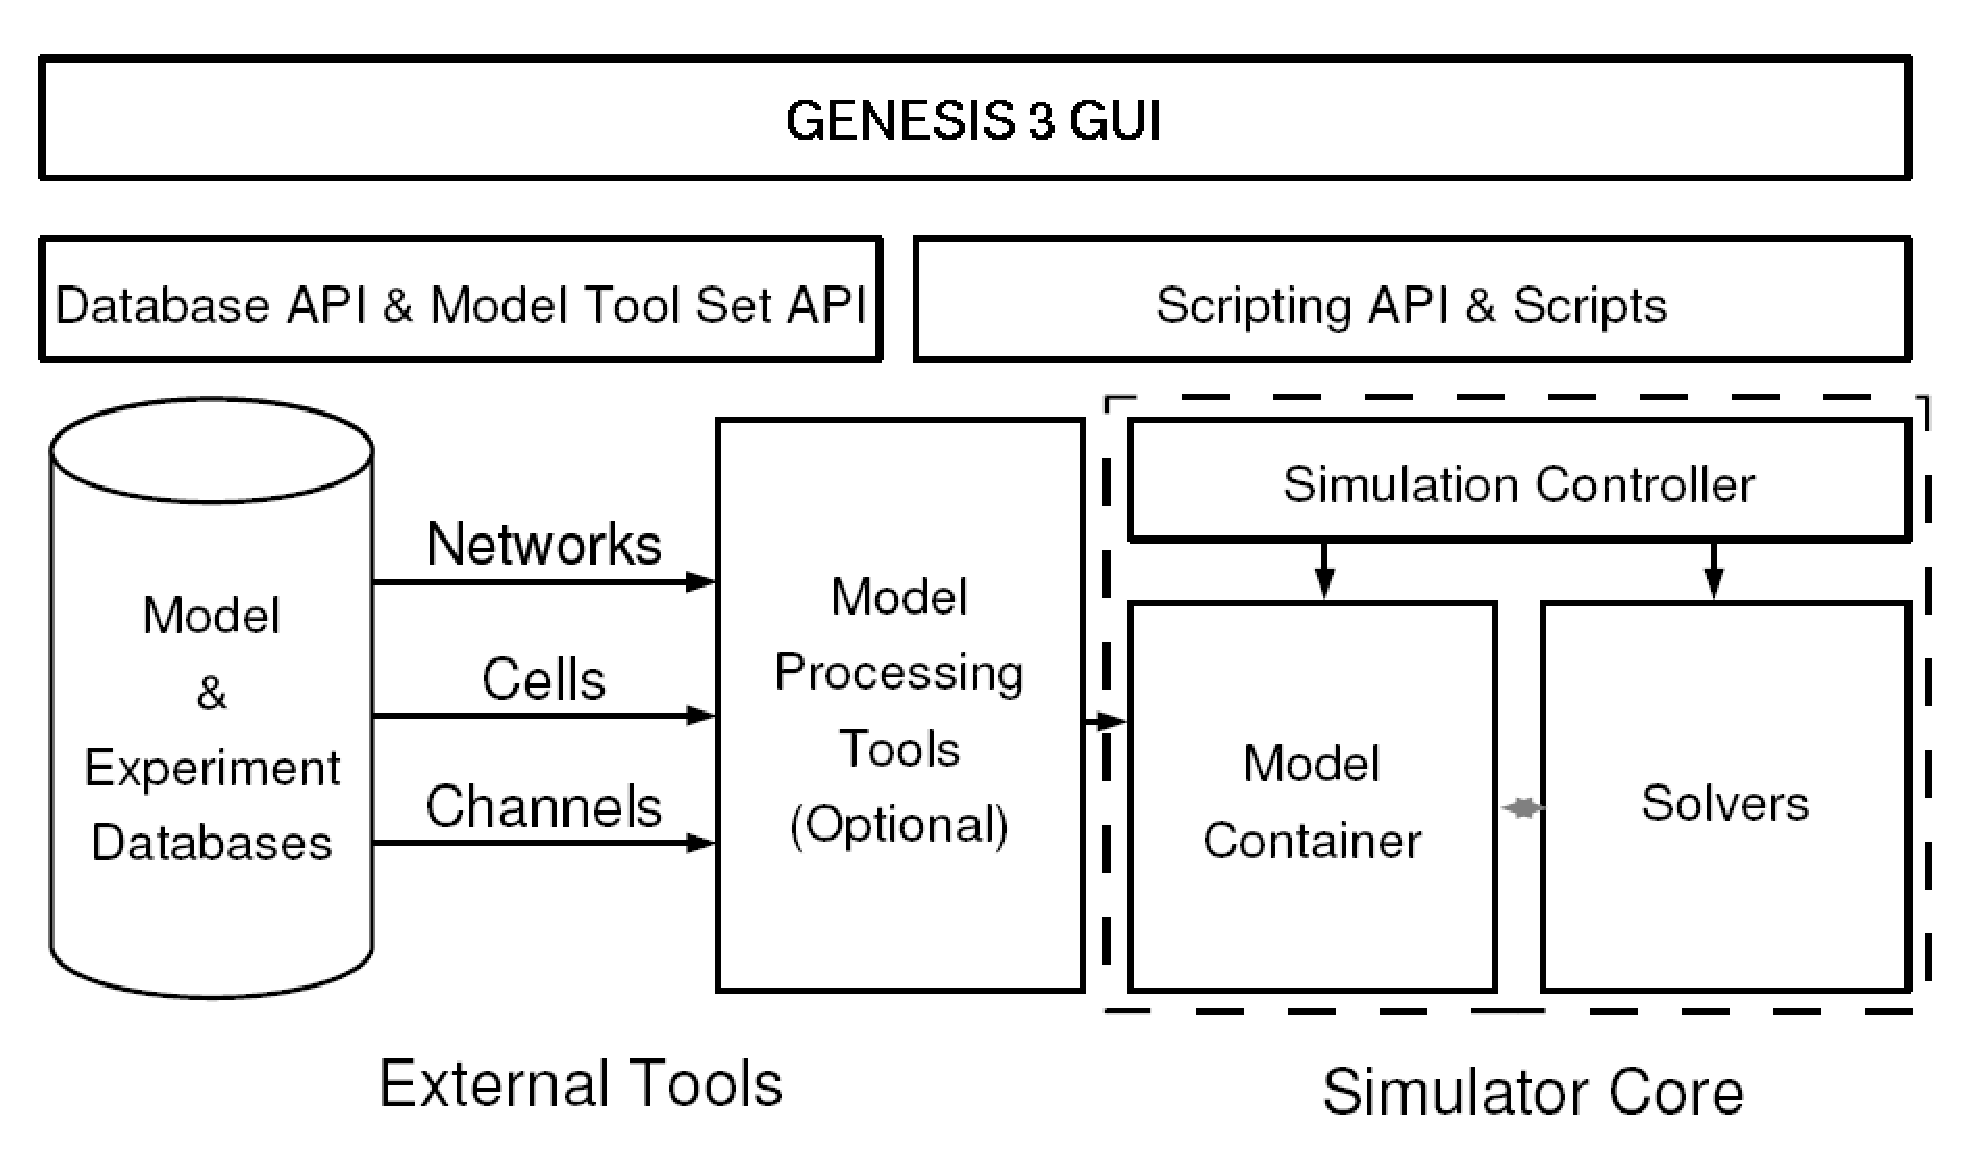
\includegraphics[scale=0.4]{figures/G3arch.eps}
  \caption{Relation of components in the CBI architecture.}
  \label{fig:cbi-arch}
\end{figure}

A scripting layer allows the simulation system to be driven from
multiple scripting languages. Python and Perl are currently supported, as is (for backward compatibility) the GENESIS SLI. The G-3 Graphic User Interface or GUI ({\bf G-Tube}), shown at the top of Figure~\ref{fig:cbi-arch},
is entirely developed in Python.  It allows models to be imported from
databases or constructed from scratch, the exploration of model
structure and parameters, and the visualization of variables and model
behavior.

\subsection{The CBI Federated Software Architecture}

The CBI (Computational Biology Initiative) federated software architecture
provides a modular paradigm that places stand-alone software
components into logical relationships. Each software module is an independent and standalone component such that development and maintenance can be implemented concurrently. This leads to a federated software architecture that exists as an ecology of software components that are CBI compliant. In this it shares a number of
ideas with the well-known three-tier architecture paradigm.  The
distinguishing feature of the CBI architecture is that the back end
comprises mathematical solvers rather than relational databases.  The
data layers in the CBI architecture correspond to high-level data
associated with biological concepts and extend to low level data such
as numerical values. The benefit of this layering of data is that it
allows the mathematical and biological aspects of a model to be
distinguished and separated.

Clear delineation of the components in the CBI architecture allows both
developers and users to choose to contribute to a single component
with limited complexity, instead of being forced to contribute to the
whole simulator and be exposed to tremendous complexity. Within the
CBI paradigm each software component is self contained and can be run independently. This facilitates the
interoperability of software obtained from different sources and has
several important advantages, including: (1) reduced complexity of
software components compared to a unitary system, (2) simplified
documentation of components in terms of inputs and outputs, (3) easy
incorporation or removal of individual components as required, (4)
simplified development and testing of components as stand alone
components, and (5) clear delineation of scope for the development of new
components. The federated approach provides three significant advantages
for software development: (1) components can be run separately on
different machines, for example, {\bf G-Tube} and the modeling environment
might run locally, while the mathematical solvers run elsewhere, either serially
or in parallel, on more powerful machines, (2) decomposition of an
application into multiple software components allows reuse and
extension of individual components, whether stand alone or otherwise,
clearly facilitating model development and research progress, and (3)
individual components can be independently updated, enhanced, or
replaced when needed, thus the life cycle of a modular architecture is
smoother than that of a non-scalable application.

The Neurospaces project (http://www.neurospaces.org/) provides
core software components of the G-3
simulator\,\cite{cornelis03:_neuros}. These include, (1) the {\bf Model
  Container}: Stores two representations of a model, the first is
conceptual and can be regarded as an enumeration of biological
concepts and their relationships, the second is an expanded
mathematical representation that, if complete, can be simulated, (2)
{\bf Heccer}: A fast compartmental solver based on the GENESIS {\it
  hsolve} object that can be instantiated from C, Perl, Python or
other scripting languages, (3) {\bf SSP} (Simple Scheduler in Perl):
Binds {\bf Heccer} and the {\bf Model\,Container}, and activates them
correctly, such that they work together on a single simulation, (4)
{\bf Studio} and {\bf G-Tube}: Contain graphical tools for model
construction, exploration and simulation, (5) {\bf G-Shell} (G-3 interactive Shell):
Dynamically loads other software components in an interactive
environment, and the (6) {\bf Project\,Browser}: For inspection of projects
and simulation results. For completeness we also mention (7) {\bf
  NS-SLI}: The G-3 component that provides backward compatibility for
the GENESIS 2 SLI. All software can be downloaded from the GENESIS web site
(http://genesis-sim.org/download/) and extensive installation
instructions with examples are available from the GENESIS
documentation website
(http://www.genesis-sim.org/userdocs/genesis-installation/genesis-installation.html).

Much existing software such as GUI libraries and plotting
libraries, are application neutral.  Other software packages are
tailored to the needs of computational neuroscience.  The CBI federated
software architecture provides a framework for integration of a functioning
simulator using a scripting language, web services and other
integration technology.  Thus, the software architecture provides
an extremely plastic environment within which independent components can
be integrated with scripting languages of choice.  Here we
specifically illustrate the use of Perl and Python for this purpose.

\subsection{Perl}

Perl was one of the first open source scripting languages. First released in 1987 [http://groups.google.com/group/comp.sources.unix/msg/bb3ee125385ae25f?pli=1], it is unique in that it is very much informed by linguistic principles. Originally developed as a scripting language for UNIX, it aimed to blend the ease of use of the UNIX shell with the power and flexibility of a system programming language like C. With over 20 years of development and nearly half a million lines of code, Perl now runs on over 100 different platforms [ref: http://www.perl.org/about.html]. Currently, there are over 18,000 open source modules available from the Comprehensive Perl Archive Network (CPAN). Perl source code has been certified to contain 0.03 defects per 1000 lines of code [http://scan.coverity.com/rung2.html]. In December 2009, nearly 2.7\,\%of all lines of programming code were written in Perl to make it the 9th most popular programming language\,\cite{software09:_tiobe_progr_commun_index}.

\subsection{Python}

Python is a powerful dynamic programming language comparable to Perl,
Ruby, or Scheme.  In December 2009 nearly 5.2\% of all code written was
developed in Python to make it the 7th most popular programming
language\,\cite{software09:_tiobe_progr_commun_index}. It combines
considerable power with very clear syntax and has modules, classes,
exceptions, and high level data types, in combination with a dynamic
and loose typing. It runs on many hardware architectures, integrates
with scientific and user interface libraries, and new modules are
easily written in C or C++ (or other languages, depending on the
chosen implementation). It is also usable as an extension language for
applications written in other languages that need easy-to-use
scripting or automation interfaces.

% 9. http://www.tiobe.com/index.php/content/paperinfo/tpci/index.html.

\subsection{Meta-Programming in Perl and Python}

Meta-programming is a programming technique where a program generates
a new program and then executes it.  We used this technique for the G-3
Python bindings to generate an additional layer of Python code that
provides increased flexibility for the definition of models and
simulations.  The key Python primitive used is a data structure that
defines high-level interfaces.  During program initialization this
data structure is translated into strings containing Python code such as
class and method definitions. These, in turn, are then bound to the run-time
environment using the Python\,{\it eval} function.

\subsection{SWIG for Federated Software Integration}

SWIG was chosen to facilitate the use of Perl and Python bindings in G-3. It is
a software development tool that connects programs written in C and
C++ with high-level scripting languages, such as Python and Perl. For
the CBI architecture, it provides control over most aspects of wrapper
generation and automates the generation of the required Python
interfaces. SWIG uses a layered approach to build Python extension
modules where different parts are defined in either C or
Python. The C layer contains low-level wrappers whereas the Python
code is used to define high-level features.  Considerably more
flexibility is obtained by generating code in both languages as an
extension module can be enhanced with support code in either language.
Table~\ref{tab:cbi-codecounts} gives an overview of the resulting
code.  As expected, low-level software components emphasize
low-level languages and have more lines of code, whereas, high-level
software components emphasize high-level languages and have fewer lines
of code.

\begin{table}[h]
  \centering
  \begin{tabular}{|l|c|c|c|c|c|c|}
    \hline

    \rule[-2ex]{0mm}{5ex}
    {\bf Language:}
    & {\bf C (H)}
    & {\bf C (G)}
    & {\bf Perl (H)}
    & {\bf Perl (G)}
    & {\bf Python (H)}
    & {\bf Python (G)} \\

    \hline

    \rule[-2ex]{0mm}{5ex}
    {\bf Model\,Container}
    & 1,832,580
    & 4,416,163
    & 30,406
    & 207,638
    & 14,568
    & 250,178 \\

    \rule[-2ex]{0mm}{5ex}
    {\bf Heccer}
    & 1,163,991
    & 1,575,615
    & 57,565
    & 107,261
    & 1,586
    & 171,219 \\

    \rule[-2ex]{0mm}{5ex}
    {\bf NS-SLI}
    & 1,448,636
    & 483,641
    & 4,603
    & 2,802
    & ---
    & --- \\

    \rule[-2ex]{0mm}{5ex}
    {\bf SSP}
    & 829
    & 2,323
    & 55,063
    & ---
    & ---
    & --- \\

    \rule[-2ex]{0mm}{5ex}
    {\bf Studio}
    & ---
    & ---
    & 174,923
    & ---
    & ---
    & --- \\

    \rule[-2ex]{0mm}{5ex}
    {\bf G-Shell}
    & ---
    & ---
    & 28,142
    & ---
    & 623
    & 836 \\

    \hline
  \end{tabular}
  \caption
  [Languages Used: Comparison of Hand-Written and Generated Code Counts.]
  {
    {\bf Languages Used:} Comparison of hand-written (H) and generated (G)  code character counts.
  }
  \label{tab:cbi-codecounts}
\end{table}


\section{Results}

Developed by Michael Vanier in the late 1990's, PyGENESIS was a
version of GENESIS that replaced the standard GENESIS SLI with a
Python interface\,\cite{vanier97:_genes_python}.  This Python-enabled
version of GENESIS was never publicly released due to the then
immaturity of Python as a scripting language.  However, with the
current sophistication of the Python platform and development of G-3
as a federated software architecture, Python interfaces have been
developed for several of the simulator core components.  While it is
possible to drive each component in isolation from these interfaces,
in the next sections, we focus on how they may be integrated to create
a simulator with a user-friendly interface.

\subsection{A Python Enabled Neural Simulator}
\label{ss-apens}

Python uses modules to group related functions together.  The G-3 Python
bindings use modules to separate interfaces for
simple models with many default settings (e.g. to start a new research
project) from more complicated interfaces that expose the full
functionality of the simulator.

As an example the {\it Neurospaces.SingleCellContainer} module
contains functions to simplify the simulation of single neuron models.
This module is a front-end to the {\it Neurospaces} module.  {\it
  Neurospaces} interfaces with the {\bf Model\,Container} which is coded in
an efficient system programming language.  Likewise, {\it
  Heccer.SimpleHeccer} is a wrapper module around the {\bf Heccer}
component which in turn is an interface to the low-level single neuron
solver.  Other components are under construction to facilitate network
modeling.

Here we show a simple high-level Python script\,\footnote{The given code
  is written for clarity of the paper rather than for compactness or
  efficiency with relation to the scripting language used.} that runs
a simulation of a single cylindrical segment defined by standard
values for the parameters of membrane and axial resistance and
membrane capacitance ({\tt RM}, {\tt RA},
%\footnote{The solver requires {\tt RA} for all
%  compartments.}
and {\tt CM}, respectively).  These parameters are given by their
specific values as commonly reported in the literature, instead of
their actual values scaled to the compartment surface area as used by
a mathematical solver\,\cite{cornelis04:_neuros_param_handl}. This
script runs a single simulation, but it can also be imported as a
Python module, thus allowing access to the function {\it
  run\_simulation}.  We call this Python module {\it example}.

{\vspace*{1mm}
 { \footnotesize
  \linenumbers
  {\begin{verbatim}
#!/usr/bin/python
# load the SingleCellContainer library
import sys
sys.path.append('/usr/local/glue/swig/python')
import Neurospaces.SingleCellContainer

# A function to run a simulation.

def run_simulation(simulationtime):
   
    # create a cell for simulation
    c = Neurospaces.SingleCellContainer.Cell("/cell");

    # create a cylindrical segment inside the cell, and set its properties
    s = Neurospaces.SingleCellContainer.Segment("/cell/soma");

    s.parameter("Vm_init", -0.0680)
    s.parameter("RM", 1.000)
    s.parameter("RA", 2.50)
    s.parameter("CM", 0.0164)
    s.parameter("ELEAK", -0.0800)

    s.parameter("DIA", 2e-05)
    s.parameter("LENGTH", 4.47e-05)

    # first example: apply current injection to the soma
    s.parameter("INJECT", 1e-9)

    # second example: use a wildcard to activate endogenous synapses
    Neurospaces.SingleCellContainer.query("setparameterconcept spine::/Purk_spine/head/par 25")
    Neurospaces.SingleCellContainer.query("setparameterconcept thickd::gaba::/Purk_GABA 1")
    
    # redirect output to the given file
    Neurospaces.SingleCellContainer.set_output_filename("/tmp/output")
    
    # compile the model
    Neurospaces.SingleCellContainer.compile("/cell")
    
    # define the output variables
    Neurospaces.SingleCellContainer.output("/cell/soma", "Vm")
    
    # run the simulation
    Neurospaces.SingleCellContainer.run(simulationtime)

# The main program executes a simulation of 0.5 seconds.
# The if statement allows this file to used as an executable script and as a library.

if __name__ == '__main__':
    run_sumulation(0.5) 
\end{verbatim}
  \vspace*{1mm} }}}

Due to the CBI federated software architecture, the G-3 platform provides many user
interfaces.  As an example, the compartmental solver {\bf Heccer} can be driven
stand-alone from C code, from Python, or from Perl to run the simplest
models, or it can be integrated with the {\bf Model\,Container} for
running more realistic multicompartment models based on morphological
data.  To illustrate this flexibility we now compare the above Python
script with alternative implementations in C and the GENESIS 2 SLI.

There is an abundance of low level detail in the C code that
interfaces directly to the solver.  For example compartments are
identified by their position in an array, and parameters such as {\tt
  RM} and {\tt CM} must be provided as an ordered sequence of their
actual values (scaled to the compartment surface area).

The complexity of the GENESIS SLI interface falls between that of the
Python and Perl interfaces, and the C code interface.  While compartments have
names, parameter values are given in a format used by solvers.

%\begin{figure}[ht]
%  \centering
{\vspace*{3mm} \footnotesize
  \begin{minipage}{1\linewidth}
    
    \begin{minipage}[t]{.50\linewidth}
{\bf C Code Implementation}
\resetlinenumber
\begin{verbatim}
#include "heccer/compartment.h"
struct Compartment compSoma =
{
 // type of structure
 { MATH_TYPE_Compartment, },

 -1,  // no parent compartment
 4.57537e-11, // Cm
 -0.08,       // Em
 -0.068,      // InitVm
 1e-9,        // Inject
 360502,      // Ra
 3.58441e+08, // Rm
};

//  compartment and channel mapping
int piC2m[] = { 0, -1, };

// model definition
struct Intermediary inter =
{ 1, &compSoma, NULL, piC2m, };

// main simulation script
#include "main.c"

\end{verbatim}
    \end{minipage}
    \begin{minipage}[t]{.50\linewidth}
{\bf GENESIS 2 SLI Implementation}
\resetlinenumber
\begin{verbatim}


create neutral /cell
create compartment /cell/soma

setfield /cell/soma dia 2e-05
setfield /cell/soma len 4.47e-05

setfield /cell/soma Cm 4.60608e-11
setfield /cell/soma Em -0.0800
setfield /cell/soma Vm_init -0.068
setfield /cell/soma Ra 355711
setfield /cell/soma Rm 3.56051e+08

setfield /cell/soma inject 1e-9







reset
step 0.5 -time
\end{verbatim}
    \end{minipage}
%    \begin{minipage}{.50\linewidth}
%\begin{verbatim}
%Compare GENESIS SLI \& G-3 C code \& G-3 perl \& G-3 Python
%\end{verbatim}
%    \end{minipage}
%    \begin{minipage}{.50\linewidth}
%\begin{verbatim}
%Compare GENESIS SLI \& G-3 C code \& G-3 perl \& G-3 Python
%\end{verbatim}
%    \end{minipage}
  \end{minipage}
  \linenumbers
  \vspace*{1mm}
}
%\end{figure}

While Python bindings are suitable for construction of toy models from
scratch, it is better to use a domain specific language to construct
the various parts of a model. For example, the {\bf Model\,Container} is
installed with a library of model components where the
standard Hodgkin-Huxley channels are provided in the file {\it
  channels/hodgkin-huxley.ndf}.  These channels can be included in the
{\it example} given above by adding the Python statements:

{\footnotesize
%  \resetlinenumber[23]
%  \linenumbers
\begin{verbatim}
   s.import_child("channels/hodgkin-huxley.ndf::/k")
   s.import_child("channels/hodgkin-huxley.ndf::/na")
\end{verbatim}
}

The {\bf Model\,Container} can export models constructed in Perl, Python or other
scripting languages as a library for incorporation into new models or
for use with other tools such as the {\bf Project\,Browser}.
These new models can then be imported by a call to the {\tt
  Neurospaces} {\it read} method. For example, importing a Purkinje
cell model with over 4000 compartments may be done with the following
statement:

{\footnotesize
\begin{verbatim}
   Neurospaces.SingleCellContainer.read("cells/purkinje/edsjb1994.ndf")
\end{verbatim}
}

The structure of the model can then be analyzed.  For example, the
names of the most distal segment of each dendrite can be obtained
with:

{\footnotesize
\begin{verbatim}
   Neurospaces.SingleCellContainer.query("segmentertips /Purkinje")
\end{verbatim}
}

\subsection{Interactive Query and Simulation}

The {\bf Model\,Container} `knows' about biological concepts such as a neuron
morphology.  From the primary morphology structure it defines derived
attributes such as total cell volume and the number of somatopetal
branch points given the name of a dendritic segment.

The {\bf G-Shell} integrates other software components into an
interactive environment that can be used to explore a
model, for example structural aspects such as morphology, and to query
derived attributes such as total volume and surface area.  The {\bf
  G-Shell} is started from a UNIX system shell with:

{\footnotesize
\begin{verbatim}
   genesis-g3
\end{verbatim}
}

After the {\bf G-Shell} has been started, the command:

{\footnotesize
\begin{verbatim}
   ndf_load cells/purkinje/edsjb1994.ndf
\end{verbatim}
}

will load the given file with a declarative specification of a
cerebellar Purkinje cell.

Alternatively, if the model is encoded in a GENESIS 2 SLI script the
command {\it ndf\_load} can be replaced with {\it sli\_load}:

{\footnotesize
\begin{verbatim}
   sli_load PurkM9_model/CURRENT9.g
\end{verbatim}
}

This command imports the model that is specified in the SLI script
without running the simulation.  A similar command is provided to
interface with the PyNN network modeling
environment\,\cite{andrew08:_pynn}.

Given the name of one of its dendritic segments, the number of branch
points between that segment and the soma can be determined. After
indicating which paths of the dendritic tree must be examined, the
parameter {\tt SOMATOPETAL\_BRANCHPOINTS} contains the result, which
can be obtained with:

{\footnotesize
\begin{verbatim}
   morphology_summarize /Purkinje
   show_parameter /Purkinje/segments/b1s06[182] SOMATOPETAL_BRANCHPOINTS
\end{verbatim}
}

After finding a suitable dendritic segment, a given synaptic channel can
be stimulated with a precomputed spike train that is stored in a file
with, for example, the filename {\it event\_data/events.yml}:

{\footnotesize
\begin{verbatim}
   set_runtime_parameter /Purkinje/segments/b1s06[182]/Purkinje_spine_0/head/par/synapse
      EVENT_FILENAME ``event_data/events.yml''
\end{verbatim}
}

Finally, following the addition of an output comprising the somatic membrane potential, a simulation can conveniently be started using:

{\footnotesize
\begin{verbatim}
   add_output /Purkinje/segments/soma Vm
   run /Purkinje 0.1
\end{verbatim}
}

This outputs the somatic response to the stimulus in a file named by default as {\it /tmp/output}.

To query the parameters of the stimulated compartment the model can
then be analyzed using the graphical front-end of the {\bf Studio}
with the command:

{\footnotesize
\begin{verbatim}
   explore
\end{verbatim}
}

\begin{figure}[ht]
  \centering
  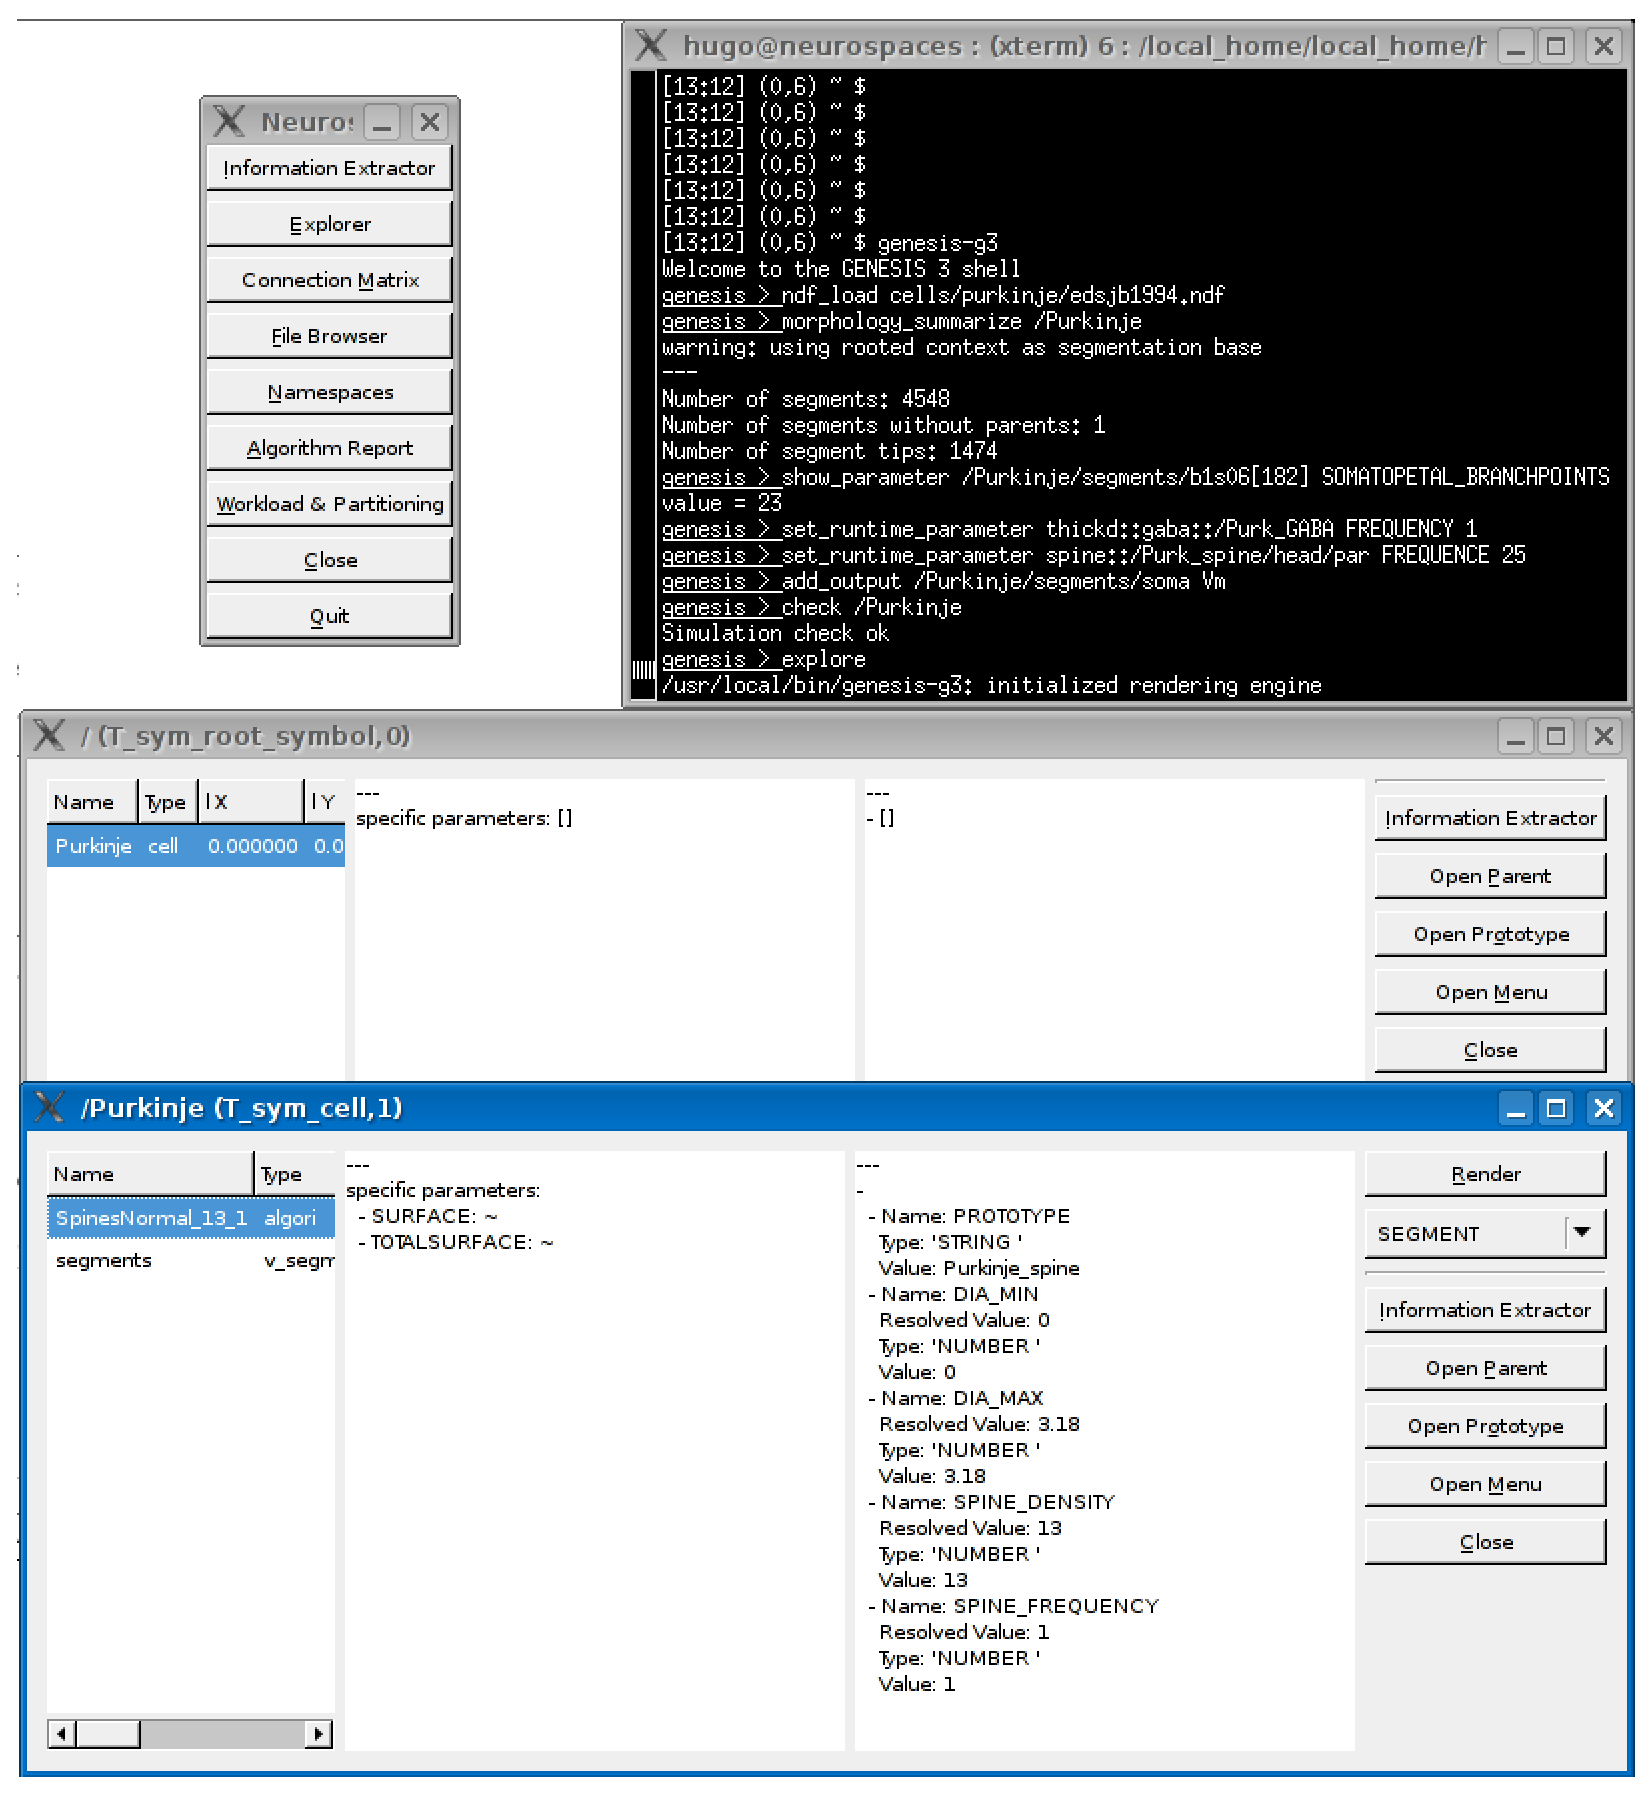
\includegraphics[scale=0.3]{figures/studio-screenshot.eps}
  \caption{Using the {\bf Studio} to query a model and its
    parameters.}
  \label{fig:cbi-studio}
\end{figure}

Figure~\ref{fig:cbi-studio} shows sample output of running this
command.  Other capabilities of the {\bf Studio} include rendering
morphologies in three dimensions and generating overviews of network
models (not shown).  In the next section we explore more graphical
capabilities of G-3.

\subsection{Gluing Pre-existing Applications \& Libraries}

In the past, the graphical interface to GENESIS 2 was provided by the
X-Window System Output and Display Utility for Simulations (XODUS).  The
XODUS interface made graphical objects available that could be
connected to model components from within the SLI.  Rather than
providing a full GUI instance, the flexibility of XODUS came from its
infrastructure which allowed modelers to easily develop new GUIs
dedicated to their research and teaching projects\,\footnote{The
  official GENESIS 2 software distribution contains both simple and
  sophisticated example GUIs.}.  However, the XODUS paradigm
inevitably allowed modelers to contaminate their model script with GUI
related statements.
%\marginpar{this is a new paragraph: problem statement to
%  introduce new G3 GUI capabilities}.

As mentioned above, one advantage of the CBI federated software
architecture is that it defines how to interface simulator components
with external applications.  An obvious example is the use of existing
3D graphics software to examine and edit the spatial properties of a
model neuron morphology.  Others include, integration with external
graphing and windowing software to plot the values of solved
variables against simulation time, or to allow the construction of
button-rich tutorial applications.

%The events that are
%generated inside such a GUI application fall into one of two
%categories.  The first, considers events generated to open a menu or
%dialog interface.  The second, considers events that interact with the
%simulation.  Since a lot of documentation for the former is available
%on the internet, we only deal here with the latter, and focus on
%events such as starting and stopping a simulation.
GUI libraries typically communicate with other software components
using an event based system.  The functional core of this system is an
event dispatching loop, usually called the {\it main\,loop}.
%How to
%setup communication between a main loop and simple actions such as
%starting and stopping a simulation is specific to the GUI library.
Both the binding between button click and event, and the visual layout
of most contemporary GUI applications is conveniently constructed
using one of a number of available user interface builders.
Additional bindings are required to implement the bindings for
simulator specific events such as starting and stopping a simulation.

We are currently working on integration of the G-3 platform and the
freely available {\it wxWidgets} library and its Python module {\it
  wxPython}.
% commented out Wednesday, Dec 2, 2009
%
% The script now handles the plotting on it's own via the DataPlot class,
% So this sentence doesn't apply anymore
%
%A Python interface to a 2D plotting library ({\it
%  matplotlib}) can be used to produce publication quality figures in a
%variety of hardcopy formats.
We also employ {\it wxFormBuilder}\,\footnote{A user interface
  designer for the {\it wxPython} toolkit and the Linux desktop
  environment GNOME, available from http://wxformbuilder.org/.} which
allows a user to construct a GUI with visual elements such as menus
and buttons, and write a description of the elements to a file
readable via Python bindings known as an XML Resource File (XRC).
Additional G-3 specific data bindings ensure that, for example, the
data produced by a mathematical solver flows to a widget that plots
the value of a variable against time.  This functionality replaces the
GENESIS 2 XODUS paradigm that required SLI scripting to connect GUI
components to model components and simulation actions, with a
contemporary paradigm that separates simulator and model scripts from
GUI related statements.

In the following example we create a {\it wxPython} application class
called {\it G3App} which demonstrates the Python scripting needed to
connect software components required to build a small GUI for
G-3.  We specifically show how to initialize the application
(implementation of method {\it OnInit}), how to run a simple
simulation (method {\it OnRun}), and how to plot output (method {\it
  Plot}).  For this, it is assumed that a XRC file with the name {\it
  G3.xrc} can be found that describes a GUI with one frame (here, {\it
  mainFrame}) which allows the simulation duration to be set via a
text control and contains a button to start the simulation.

The first lines of code in the script load the necessary Python
modules which then load low-level libraries coded in a system
programming language.  The importation of {\it example} makes the
previously defined function {\it run\_simulation} available.  The {\it
  DataPlot} class is a specialized class to read in GENESIS data
output and load it into a {\it wxPython} plot widget.  The import for
{\it wx} references a system wide install of {\it wxPython} and makes
the GUI functions of {\it wxWidgets} available to our script.

{\footnotesize
%  \resetlinenumber
  \linenumbers*
\begin{verbatim}
import DataPlot
import example
import wx
from wx import xrc
\end{verbatim}
}

To ensure correct system initialization via the method {\it OnInit},
our {\it G3App} class is declared to inherit the functions of the {\it
  wx.App} class.

{\footnotesize
\linenumbers
 \begin{verbatim}
class G3App(wx.App):

    def OnInit(self):
 \end{verbatim}
}

After correct system initialization, application specific
initialization can start.  Inside the {\it OnInit} method we first
load the XML resource file previously created using {\it
  wxFormBuilder}.

{\footnotesize
   \linenumbers
 \begin{verbatim}
        self.res = xrc.XmlResource('G3.xrc')
 \end{verbatim}
}

The GUI elements are then retrieved from the XRC specification and
made available as Python objects.  Each declared object can be
retrieved via its name:

{\footnotesize
   \linenumbers
 \begin{verbatim}
        self.frame = self.res.LoadFrame(None, 'mainFrame')
        self.runButton = xrc.XRCCTRL(self.frame, 'runButton')
        self.durationTextCtrl = xrc.XRCCTRL(self.frame,'durationTextCtrl')
 \end{verbatim}
}

After retrieving the run button, we bind it to the method {\it OnRun}
(given below).  This translates the GUI event generated when
the run button is clicked to an action that invokes the {\it OnRun}
method.

{\footnotesize
   \linenumbers
 \begin{verbatim}
        self.frame.Bind(wx.EVT_BUTTON, self.OnRun, self.runButton)
 \end{verbatim} 
}

% The following Python code reads the Glade XML file and connects a
% button with a function to run the simulation:

% {\footnotesize
%   \resetlinenumber[5]
%   \linenumbers
% \begin{verbatim}
% wTree = gtk.glade.XML("G3.glade", "window1")
% wTree.signal_autoconnect( { "on_button1_clicked": run_simulation } )
% \end{verbatim}
% }

% Tuesday, Dec 1, 2009
%<--- start
% simplified the gui so this button is no longer needed. 
% 
% The function {\it OnSet} 
%is fairly simple, its only purpose is to read the value in the 
%user input text control ({\it self.durationTextCtrl}) and pass this value
%to a global variable called {\it simulation\_time}.

%{\footnotesize
%  \resetlinenumber[12]
%  \linenumbers
%\begin{verbatim}
%   def OnSet(self, evt):
%      global simulation_time
%      simulation_time = float(self.durationTextCtrl.GetValue())
% \end{verbatim}
%}
%end --->

The {\it OnRun} method reads a numerical value for the the simulation
time from a text control widget ({\it durationTextCtrl}) and stores it
in a variable.  This variable is then passed to the function {\it
  run\_simulation}.  After the simulation is complete a call to a {\it
  Plot} method is made. This displays the generated data in a {\it
  wxPython} plot widget.

{\footnotesize
  \linenumbers
\begin{verbatim}
    def OnRun(self,evt):

        simulation_time = float(self.durationTextCtrl.GetValue())
        example.run_simulation(simulation_time)
        self.Plot('/tmp/output')
\end{verbatim}
}
 
%        print "Simulation time is: " + str(simulation_time)
%        print "running simulation..."

%        print "Simulation Complete!"

%        print "Plotting output"

The {\it Plot} method uses the {\it DataPlot} class to display G-3 data
output with a {\it wxPython} plot widget.  The {\it DataPlot} widget
is part of the libraries of the {\bf G-Tube}, a Python GUI under
development for G-3.

{\footnotesize
  \linenumbers
\begin{verbatim} 
    def Plot(self,datafile):

        plotwindow = wx.Frame(self.frame, -1, "Graph display", (480,300))
        plotpanel = wx.Panel(plotwindow, -1)

        self.dataplot = DataPlot.DataPlot(plotpanel, -1,
                                          '/tmp/output',
                                          'Example Plot',
                                          'Time (Seconds)',
                                          'Membrane Potential (Volts)')

        vbox_sizer = wx.BoxSizer(wx.VERTICAL)
        vbox_sizer.Add(self.dataplot, 1, wx.EXPAND)
        plotpanel.SetAutoLayout(True)
        plotpanel.SetSizer(vbox_sizer)
        plotpanel.Layout()
        plotwindow.Show()
\end{verbatim}
}

The code of the GUI application ({\it G3App}) is terminated with a
call to the main event loop of {\it wxPython}.

% {\footnotesize
%   \resetlinenumber[14]
%   \linenumbers
% \begin{verbatim}
% gtk.main()
% \end{verbatim}
% }

{\footnotesize
  \linenumbers
\begin{verbatim}
if __name__ == '__main__':
    app = G3App(False)
    app.MainLoop()
\end{verbatim}
}

% Tues, Dec 1, 2009
%
% Code is no longer valid, translated this to the wx.lib.plot
% implementation. Moved it before the call to the main loop since 
% the plot call is now part of the G3App class. 
%
%<-- start

%This script runs a small model and can be combined with other Python
%code given here to increase the complexity of a model, add various
%stimulus conditions, and extract the output of interest.  The script
%saves the membrane potential of the soma to the file {\it
%  /tmp/output}.  To plot this membrane potential in the application
%window, the {\it matplotlib} library is used:

%{\footnotesize
%  \resetlinenumber[5]
%%  \linenumbers
%\begin{verbatim}
%   import matplotlib
%   import pylab
%\end{verbatim}
%}

%The following code reads the output file into two arrays, {\it t} and
%{\it v}\footnote{The given code is written for clarity of the paper
%  rather than for compactness or efficiency with relation to the
%  scripting language used.  For example here a single call to the
%  builtin function numpy.loadtxt() could have been used.}:

%{\footnotesize
%  \resetlinenumber[5]
%%  \linenumbers
%\begin{verbatim}
%   t = []; v = [] ;
%      file = open("/tmp/output")
%      for line in file:
%         values = re.split(" ", line)
%         t.append(float(values[0]))
%         v.append(float(values[1]))
%\end{verbatim}
%}

%The plot widget is not directly supported by Glade and must be created
%with custom Python code.  A plot can then be generated using:

%{\footnotesize
%  \resetlinenumber[5]
%%  \linenumbers
%\begin{verbatim}
%   # generate the plot
%   figure = matplotlib.figure.Figure(figsize=(6,4), dpi=60)
%   axis = figure.add_subplot(111)
%   axis.plot(t,v)

%   # display the plot
%   canvas = matplotlib.backends.backend_gtk.FigureCanvasGTK(figure)
%   canvas.show()
%   grahview = wTree.get_widget("vbox1")
%   grahview.pack_start(canvas, True, True)
%\end{verbatim}
%}

%end --->

In this example we have shown how the CBI architecture allows for
separation between GUI statements and peripheral code such as input
and output specifications, and model construction.  Besides allowing common GUI construction kits to be used for the development of
research and educational projects, the approach also allows interfacing to more specialized GUI kits.  This is illustrated with the following example.

\subsection{Interfacing GENESIS with Blender}

% Another possible example is that of integration
%of the {\bf Model\,Container} with a web server to allow measurement
%and analysis of morphologies in a morphology database.  Such a
%platform would likely be useful, for example, for the neuro-morpho
%database\,\cite{ascoli06:_mobil, ascoli07:_neurom}.

Blender (http://www.blender.org/) is a free open source 3D content
creation suite available for all major operating systems that have
Python enabled bindings.  The Python environment of Blender has the
restriction that the code must be run from inside the Blender specific
Python interpreter. In doing this, Blender replaces the functionality otherwise
provided by the {\bf G-Shell}. It allows the state-of-the-art rendering
functions of Blender to be used to validate and analyze models of the morphology
of small dendritic segments obtained from electron microscopy data.

Past research has shown that the balance
between excitation and inhibition plays an important role in dendritic
processing in cerebellar Purkinje cells\,\cite{santamaria02:_modul_purkin,
  mittmann07:_linkin_purkin}.  However, the spatial resolution of the
models employed in such studies was limited by the available reconstruction
techniques.  To overcome this problem, over the last several years
we have used electron microscopy in conjunction with
Reconstruct\,\cite{jc05:_recon} to obtain more precise morphologies of
small segments of Purkinje cell dendrites\,\cite{huo09:_purkin,
  cornelis08:_model_neuros_genes}).

\begin{figure}[ht]
  \centering
    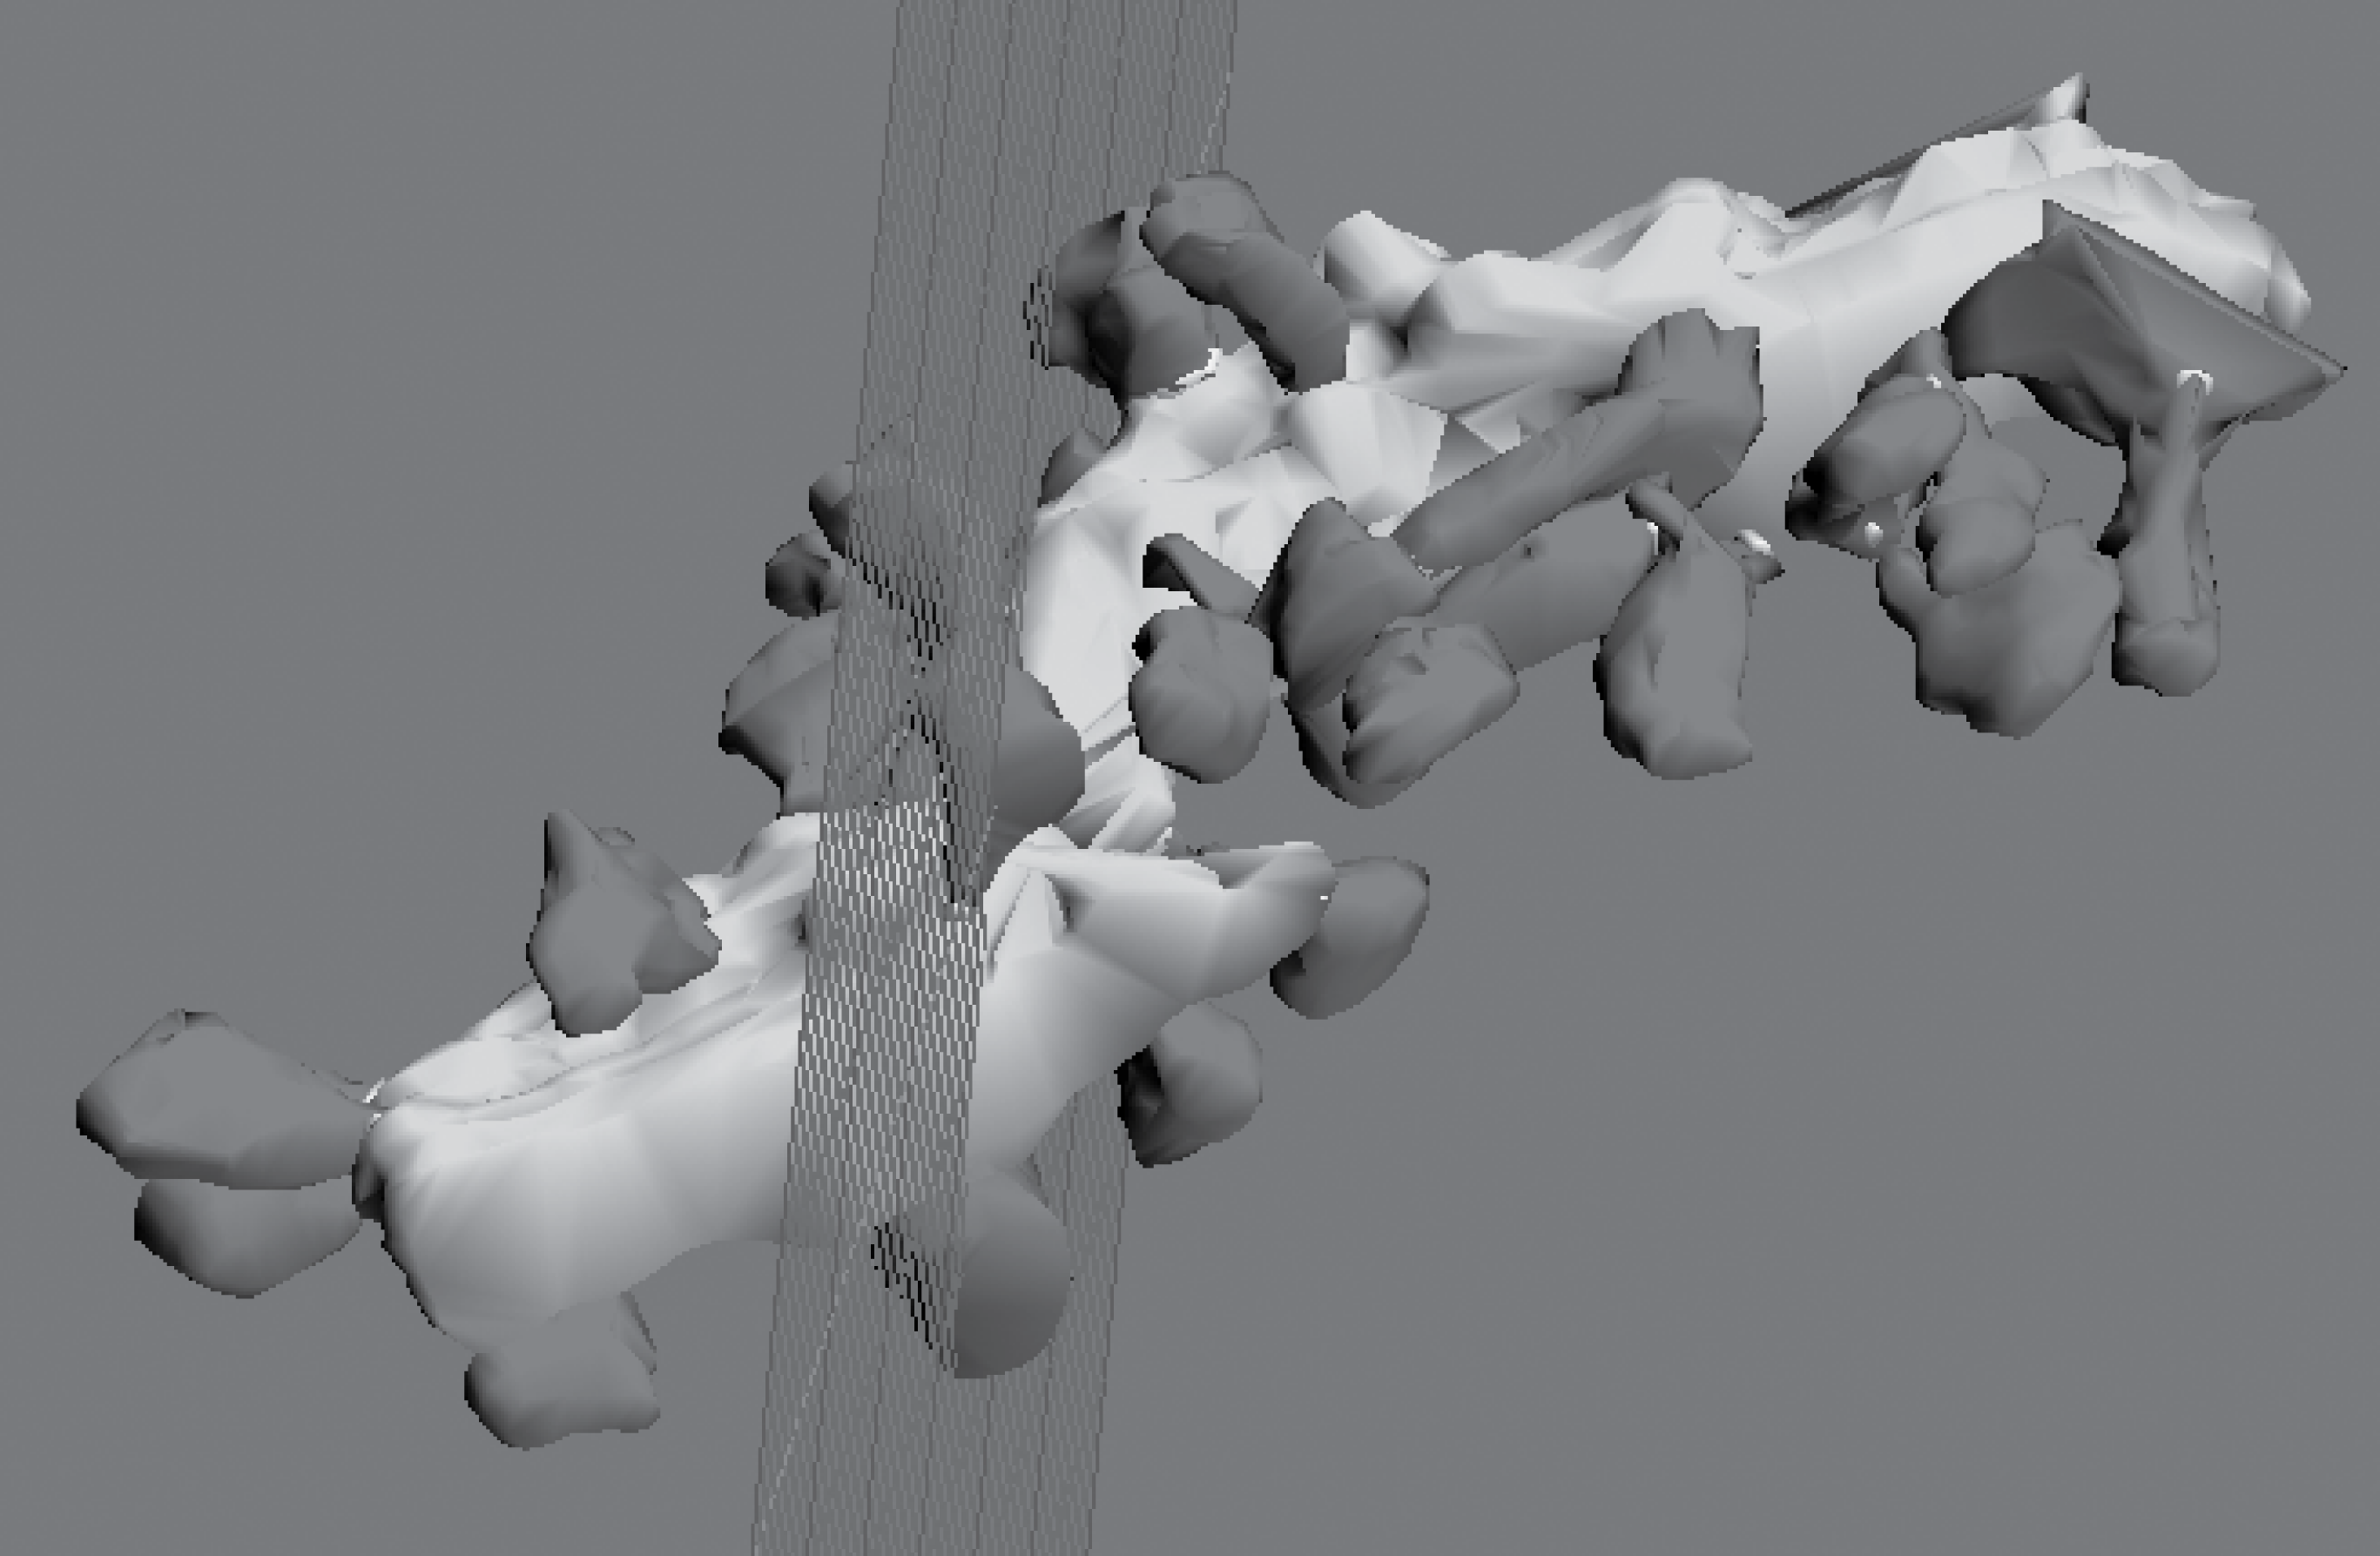
\includegraphics[scale=0.5]{figures/blender-python-bw.eps}
  \caption{Blender image of Purkinje neuron dendritic segment}
  \label{fig:cbi-blender}
\end{figure}

% \noindent{\bf Hugo: Show Python interface snippet.}

Special purpose software has been written to convert Reconstruct data
for importation into the {\bf Model\,Container}.  The {\it
  Reconstruct\,Interface} converts the Reconstruct application into a
G-3 simulator component by making it CBI compliant.
%  It converts
%contours exported by the Reconstruct software to the declarative NDF
%format (the file format used by G-3). 
The core of this interface implements geometrical transformation
algorithms that convert EM contours provided by Reconstruct to
equivalent cylinders suitable for cable modeling.
% The core of these algorithms
%implements geometrical transformations such that EM contours are
%extracted to provide equivalent cylinders suitable for cable modeling.
The geometrical properties of the cylinders are stored in the native G-3 file format as NDF files. Algorithms provided by the {\bf Model\,Container} link them with
the cable parameters required by the mathematical solvers.  A
simulation can then be run with the {\it read} and {\it run} methods
given above.

The necessary conversion algorithms are accessible from the
{\bf Model\,Container} via Python.  The Python interface of Blender links it to the G-3
simulator, such that Blender is the first G-3 3D model inspection
tool for EM data.  As an example, the Python script developed above
can be run from within the Blender environment.  Also, via the same
Python interface, simulations can be started based on the 3D image
data.

Interactive visualization of reconstructed dendritic segments is a
valuable method of model validation and is available with the
interface of G-3 with Blender (see Figure~\ref{fig:cbi-blender}).
However, the development of small focused plugins allows for more than
just these functions. For example, 3D measurement and manipulation of
neuron morphology, computation of surface areas and volumes, and the
generation of 3D crossections and 2D cuts also becomes possible.

\section{Discussion}

The current
generation of neural simulators can be characterized as software
applications that support a user workflow extending from model
construction to data analysis.  Many of these simulators come with
Python bindings, ranging from Monte-Carlo simulators for
reaction-diffusion systems\,\cite{wils09:_steps} and dedicated large
network simulators\,\cite{eppler08:_pynes} to the general purpose
NEURON and GENESIS simulators\,\cite{hines09:_neuron_python,
  bower98:_book_genes}.  Some of these simulators use Python because
of its ease of use\,\cite{pecevski09:_pcsim} and
simplicity\,\cite{goodman08:_brian}.  For others, interoperability can
be implemented using the NeuroML standard for model specification in
XML\,\cite{nigel01:_towar_neurom} and PyNN for simulator-independent
specification of neuronal network models in
Python\,\cite{andrew08:_pynn}.

The G-3 platform now provides an alternative approach that uses scripting to connect neuroscience specific
software to general purpose software and integrate it into a next
generation neural simulator.  The advantage is that third party software
libraries and applications become available for users, for example,
Blender, {\it matplotlib}, and Glade, among many others. This has
become possible due to the rearchitectured GENESIS software design
where G-3 now conforms to the CBI federated software architecture. In this paradigm, model parameters are stored separately from stimulation
protocols and the way simulations are run. It is the stand-alone
nature of the individual software components and the fact that they
can now easily be interfaced that facilitates continued software
development and increased user-friendliness.

\subsection{Other Software Components}

To demonstrate the power of our approach, we have interfaced G-3 with Blender. This novel software platform has been used for visual inspection and validation of
reconstructed dendrites by connecting a model to the geometrical and
analytical tools provided by the Blender plugin library.  Further, we note that it
is also possible to use Blender to instantiate neural simulations and,
for example, to collect simulation output data for movie generation.

Complementary functionality to that provided by interfacing G-3 with
Blender would be available after interfacing G-3 with {\it
  neuro}Construct (http://www.neuroconstruct.org/), a software package designed to simplify the development
of complex networks of biologically realistic
neurons\,\cite{gleeson05:_build_networ_model, gleeson07}.  Implemented
in Java, {\it neuro}Construct uses the latest NeuroML specifications
(see http://www.neuroml.org), including MorphML
(http://www.morphml.org/), ChannelML and NetworkML, can be used to
visually validate network layout and design\,\cite{crook07:_morph},
and can be connected to Python applications (e.g.  see
http://www.jython.org/). In principle this allows it to be integrated
with other simulators that have Python bindings, including NEURON and
NEST.

Finally, we note that we have developed a serial communication
framework for event delivery of action potentials to postsynaptic
targets.  Called the Discrete Event System (DES), this software
component is integrated with the mathematical solvers of G-3 using
either Perl or Python.  Because it is optimized for communication over
serial hardware, DES can be extended to support communication frameworks
for parallel hardware such as those provided by the MOOSE
simulator\,\cite{ray08:_pymoos} and the MUSIC
framework\,\cite{ekeberg08:_music_multis_coord}.

%\subsection{Future Directions}

%\cite{stewart09:_python}

%\cite{deschutter09:_review_paper_descr_neuroin_softw}.

%\pagebreak

\subsection{Implications}

Software libraries can be divided into application specific and
application neutral categories.  Through the Neurospaces project,
GENESIS now provides a series of software components specific to
neuroscience applications (G-3).  The advantage is that scripting
languages such as Python and Perl become a powerful integration tool
to connect these components to general purpose libraries for
visualization, rendering, and GUIs.
Although the Python bindings of the G-3 simulator embed the same
powerful concepts as the GENESIS SLI, their purpose is different.
While the SLI had as major goals the integration of model components,
output collection, and running simulations, the primary goal of
scripting languages such as Perl and Python has become application
integration.

A key enabling property of G-3 is that it stores model parameters
separately from stimulation protocols and the way simulations are run.
By defining clear functional
boundaries of the core software components such as the {\bf
  Model\,Container} and the mathematical solvers, we also provide
clear interfaces for integration.
%We have outlined an ecology of
%software components that are CBI compliant and that integrate with the
%G-3 simulator.

Processes of software development have traditionally been described as
either cathedral-style where there is a closed developer group under
central direction and software releases are infrequent, or
bazaar-style where the software is developed by volunteers and software
releases are done early and
often\,\cite{raymond01:_cathed_bazaar, citeulike:126678}.
%Brooks' Law and Linus' Law.
%Currently, successful open source software development 
%seems to depart on the one hand from the popular view of being the
%production of an egalitarian network of developers free from the
%hierarchal organization and central control of the ``cathederal''
%model pervasive in the commercial world and, on the other hand, also
%depart from the flat structure of the open source development
%``bazaar''\,\cite{Open-Source03theecology}.
When the cathederal-style of software development leads to a single
threaded development cycle most suitable to commercial applications,
the bazaar-style leads to multi-threaded development cycles of
applications that come in different flavours\,\footnote{A typical
  example is the family of editors based on Emacs.}.

Here, we have outlined an alternative that follows the component based
approach to open source software development (for other examples of
this approach to neural simulation
see\,\cite{schuermann09:_neuron, nordlie09:_visual}). Our
approach has given rise to an ecology of software components connected
over interfaces.  Gluing these components together can be done in a
variety of ways and we have given examples that use Perl and Python.
%Here, we have illustrated the relationship between Python and the G-3
%simulator.  We have focused on a simple but comprehensive example, the
%running of a single compartment neuron and the plotting of its
%membrane potential. The purpose is to demonstrate the advantages of
%using high-level scripting languages such as Perl and/or Python for binding the
%independent stand-alone components of G-3. In the process of achieving this goal, we have defined an ecology of holistic dynamic interactions between G-3 software components.
%It is an approach that
%simplifies the extension, modification, and customization of the
%GENESIS platform, not only for developers but also most importantly
%for users.
Employed in this way, the modularized design of the G-3 simulator
provides for progressive federated software development.

%Using Python for integration makes
%the application much more accessible to users.


% ********************** Back matter ********************************
% Bibliography
\cleardoublepage
\pagenumbering{roman}
\bibliographystyle{abbrv}
%\bibliography{DDDAS_bib_library}
%\bibliography{crest2008,Qian,DDDAS_bib_library}
\bibliography{../tex/bib/g3-refs.bib}

% ********************** End of the Document ************************
\end{document}


%%% Local Variables: 
%%% mode: latex
%%% TeX-master: t
%%% End: 
